%% ------------------------------------------------------------------------- %%
\chapter{Introdução} %Nome do capítulo.
\label{cap:intro} 

O som pode ser definido como a propagação ondulatória e mecânica em um meio elástico
ou como a excitação dos mecanismos auditivos que resultam em sua percepção~\cite{Everest}. No primeiro
caso, estamos tratando de leis puramente físicas. No segundo caso, estamos lidando com um
fenômeno psicofísico. Nesta última abordagem encontramos lugar para a música, que escapa,
portanto, às leis fatídicas dos fenômenos naturais~\cite{Roederer}. A delicada tarefa de capturar estruturas
e artifícios musicais diretamente relacionados às oscilações do som discretizado
é exatamente a tarefa proposta por este trabalho. Para isso, entendemos cabível
abordar o som em sua representação digital e dispor os resultados em fórmulas matemáticas e implementações computacionais. 


    \section{Do som ao áudio digital}

Em sua conceituação puramente física, o som é uma onda mecânica longitudinal de pressão e pode se propagar por qualquer meio material.
Embora o corpo humano possa captar sons cujas frequências estão fora da banda compreendida aproximadamente entre $20Hz$ e $20 kHz$, estas são as frequências chamadas audíveis e apreciadas pelo nosso aparelho auditivo.
 Considerada a velocidade do som no ar de $\approx 343.2\,m/s$ em condições usuais,
estes limites correspondem respectivamente aos comprimentos de onda $\frac{343.2}{20} = 17.16\,m$ e $\frac{343.2}{20000}=17.16\,mm$.

A efetiva audição humana destas vibrações consiste em um fenômeno complexo ainda sob intensa pesquisa, involvendo captações pelos ossos, estômago e orelha, além de funções de transferência da cabeça e dorso e processamento pelo sistema nervoso. Existe, no entanto, um órgão dedicado à tarefa de captura destas ondas, ao qual chamamos ouvido e cujo funcionamento decompõe o som em seu espectro senoidal antes de passar o estímulo para o sistema nervoso~\cite{Roederer}. Este papel central das componentes senoidais do som é crucial para os fenômenos musicais, o que pode ser notado tanto na composição de sons de interesse para a música, quanto nas afinações e escalas~\cite{floEsp}.

A representação do som é chamada áudio e usualmente usamos este termo para designar uma representação elétrica do som\footnote{Embora haja esta tendência e tradição de uso, os termos
som e áudio são, na verdade, usados de forma intercambiável.}. O áudio pode ser proveniente da captura do som por microfones ou de síntese diretamente. O áudio digital consiste na sua representação sonora através de protocolos também digitais. Alguns destes protocolos são bastante elaborados, em geral visando resultar em quantidades reduzidas de dados para facilitar armazenamento e transferência dos arquivos. Outras representações digitais do som são bastante diretas, consistindo em amostras igualmente espaçadas no tempo e cujas amplitudes individuais são registradas com um mesmo número de bits. Esta representação do som por amostras separadas por intervalos regulares $\lambda_a$ é a forma padrão de representação do som em tempo discreto e é chamada de modulação por código de pulsos (denotada pela sigla PCM do inglê Pulse Code Modulation).
Um som digital PCM é caracterizado pela frequência de amostragem $f_a=\frac{1}{\lambda_a}$ (também chamada de taxa de amostragem) e profundidade de bit, sendo este o número de bits utilizados para representar cada amostra. Dispomos na figura~\ref{fig:PCM} um esquema gráfico de um áudio PCM. Observe que os $2^4=16$ grados disponíveis para a amplitude de cada amostra junto ao espaçamento regular $\lambda_a$ introduzem um erro de quantização. Estaremos apontando as formas de lidar com o ruído causado por estes erros de quantização sempre que pertinente.


\begin{figure}[h!]
    \centering
    \caption{Som digital em modulação por código de pulsos (PCM): 25 amostras representadas por 4 bits cada uma.}
        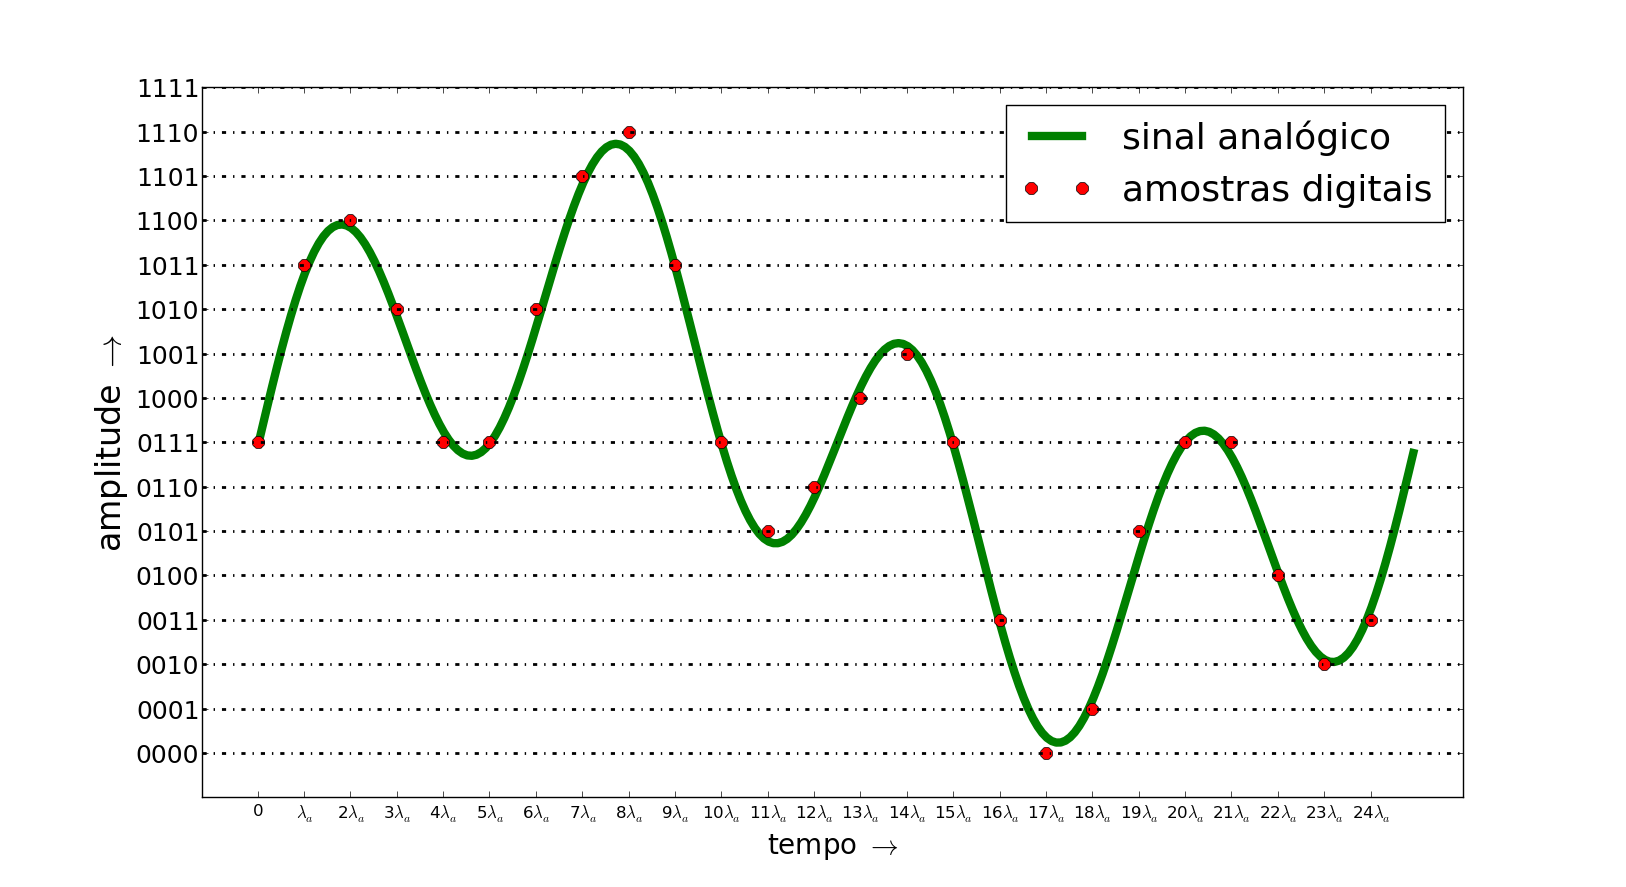
\includegraphics[width=\textwidth]{figuras/pcm}
        \label{fig:PCM}
\end{figure}

Nesta representação, é de conhecimento comum pelo teorema de Nyquist que não podemos representar frequências acima da metade da frequência de amostragem. Assim, se buscamos apreender as frequências audíveis, precisamos utilizar uma taxa de amostragem que seja ao menos o dobro da frequência mais alta capturada pelo sistema auditivo $f_a=2\times 20kHz=40kHz$. Este raciocínio está na base da utilização das frequências de amostragens $f_a=44.1kHz$ e $f_a=48kHz$, ambas utilizadas amplamente e são as taxas de amostragens padrão em \emph{Compact Disks} (CDs) e em sistemas de Rádio e TV, respectivamente.

Do ponto de vista didático, é notável que praticamente todo processamento espectral sonoro seja praticável por somatórios quando tratamos do som discretizado. Estes mesmos procedimentos são obtidos por integrais quando estamos lidando com o som analógico, o que é consideravelmente mais complicado.




    \section{Arte sonora e rudimentos de teoria musical}

A música é comumente descrita como a arte manifesta pelos sons e silêncios. Embora esta definição esteja canonicamente correta, para as concepções usuais, ela está mais associada a uma ideia de arte sonora do que à música propriamente dita, pois para um ouvinte comum - e boa parte dos especialistas - uma 'música que seja música' pressupõe também a presença de uma métrica rítmica além de organizações de alturas que formem melodias e harmonias (veja sessão~\ref{notasMusica}). De qualquer forma, é importante reconhecer que a música do século XX ampliou esta concepção tradicional de música feita por notas que formam estruturas baseadas em ritmos, melodias e harmonias bem identificáveis. Isso ocorreu primeiramente na música de concerto, especialmente nas chamadas correntes eletrônica, concreta e eletroacústica. Já na década de 90 ficou claro que também a música popular, especialmente as músicas eletrônicas de dança, tinham por sua vez se desdobrado para abarcar não só os sons de altura definida e os organizações temporais bem estabelecidas dentro de métricas simples, mas também amálgamas sonoros ruidosos e disposições temporais fluídas e com sobreposições. Mesmo assim, a nota musical permanece paradigmática como 'unidade fundamental' das estruturas musicais. Além disso, as notas podem se desdobrar em sons que se desenvolvem no tempo, contemplando estes desenvolvimentos musicais recentes que foram supracitados (veja sessão~\ref{varInternas}).

A teoria musical é uma ampla área de estudos com várias abordagens divergentes e que engloba assuntos tão diversos quanto psicoacústica, convenções culturais de organização de alturas (e.g. escalas e seus usos) e formas musicais tradicionais, como a forma sonata e rondós, que consistem em estruturas paradigmáticas para uma música inteira. Neste trabalho, a abordagem deste assunto é bastante vinculada às aplicações dispostas no capítulo seguinte e estão apontadas no próprio texto mediante necessidade. Assim, não consideramos apropriado discorrer sobre estes assuntos aqui de forma independente, e para isso dispomos os títulos referenciados em nossa bibliografia. Recomendamos também o acompanhamento de um especialista, pois, na música, é comum um mesmo termo ser utilizado para designar diferentes conceitos e um mesmo conceito ser vinculado a diferentes termos, mesmo em contextos escolásticos.


    \section{Disponibilização computacional}
Os desenvolvimentos apresentados nesta dissertação incluem \emph{scripts} (i.e. pequenos programas) escritos em Python para disponibilização das tecnologias de forma explícita. Entendemos uma linguagem como o Python ou Scilab apropriada para esta tarefa
por ser de compreensão bastante simples, aproximando-se do que chamamos de pseudo-código~\cite{tutPython}. Outra faceta importante desta disponibilização é a utilização de um sistema de controle de versão para os textos, códigos e figuras. Assim, pode-se observar o desenvolvimento do trabalho e executar modificações sem tantas preocupações, pois todas elas ficam registradas individualmente e são reversíveis. Utilizamos para isso o sistema Git, tida como a segunda grande contribuição de Linus Torvals, sendo o próprio kernel Linux a primeira.

Os \emph{scripts} estão dispostos em duas versões: em Python puro, i.e. sem bibliotecas externas, e em Python com Numpy e Audiolab. Esta segunda versão executa as rotinas através de chamadas à linguagem Fortran, muito eficiente em termos de processamento computacional e, consequentemente, em termos da duração necessária para a execução dos algoritmos.

Algum código já foi transcrito para JavaScript com muita facilidade, o que torna estas contribuições potencialmente utilizáveis em navegadores bastante difundidos, como o Firefox e o Chromium.

Estas tecnologias são todas abertas, i.e. estão publicadas em licenças que permitem o uso, cópia, distribuição e utilização de quaisquer partes para geração de produtos derivados. Desta forma, os trabalhos aqui descritos estão disponíveis como parte de um repertório tecnológico livre que constitui um patrimônio da humanidade e é vinculado usualmente às comunidades de Software Livre e de Código Aberto\footnote{A comunidade e movimento chamada \emph{'Open Source'} é uma corrente que entende a publicação em licenças abertas de código computacional (e outras tecnologias) como sendo uma vantagem pragmática, possibilitando facilidades de desenvolvimento e vantagens de aprendizado e mercadológicas. A comunidade e movimento chamada \emph{'Free Software'} engloba este entendimento, mas adiciona a abordagem filosófica da liberdade e compartilhamento, e dá ênfase a isso. Ambas as correntes reforçam o entendimento de que o código computacional é o 'bem mais  precioso produzido atualmente' pois consiste em tecnologia condensada, reativa (pois executa, processa ou gera resultados), modular (pode ter partes copiadas reutilizadas eficientemente) e replicada sem custo adicional (pois a cópia de texto tem custo baixíssimo). Muito frequentemente isso tudo está disposto em poucas linhas escritas.}. Constatamos que, desta forma, facilitamos as colaborações em processos de co-autoria e geração de materiais subsequentes.

    \section{Objetivos}
   \label{sec:objetivos}
Nosso objetivo principal nesta dissertação é dispor um sistema unificado que relacione elementos básicos da música às sequências amostrais do som digital. Este conhecimento é existente, tanto que diversos softwares comerciais apresentam desenvolvimentos relacionados, mas não há uma apresentação unificada e concisa destas relações. Assim, dispomos um texto coerente em que os elementos musicais são apresentados junto às sequências temporais envolvidas. Além disso, como parte da efetiva contribuição, entregamos implementações em código computacional (Python) destas equações e \emph{scripts} que resultam em pequenas peças musicais\footnote{Ou, de forma menos pretenciosa, montagens musicais, sequências musicais.}. 

Dada esta direção bem estabelecida, consideramos alguns objetivos secundários. Em primeiro lugar, a difusão de conhecimentos em programação e compreensão do código computacional é bastante potencializada através de práticas lúdicas, no caso a música. Outro objetivo considerado é a apresentação de um arcabouço de síntese sonora e musical com controle amostral, para o qual encontramos potenciais usos em experimentos psico-acústicos e síntese em alta definição (\emph{hi-fi}). Talvez por último, buscamos apresentar estes conteúdos de forma didática, quase um verdadeiro tutorial, possibilitando uma compreensão e uso facilitados, pois os assuntos tratados são de reconhecida complexidade: processamento de sinais, música, psico-acústica, para citar somente alguns exemplos. Deste ponto de vista didático, também reconhecemos importante a apresentação deste material na forma de hipertexto, em que cada \emph{script} e exemplo sonoro/musical seja acessível junto ao material teórico.
  
